\documentclass[12pt,a4paper]{article}

% Packages
\usepackage{
    amsmath,
    amssymb,
    graphicx,
    titletoc,
    fancyhdr,
    geometry,
    babel,
    xcolor,
    enumerate,
    fix-cm,
    tocbibind,
    listings,
    float,
    enumitem,
    subcaption,
    hyperref
}

% Define colors
\definecolor{vgreen}{RGB}{104,180,104}
\definecolor{vblue}{RGB}{49,49,255}
\definecolor{vorange}{RGB}{255,143,102}

% Listings customization
\renewcommand\lstlistingname{Figura}
\renewcommand\lstlistlistingname{Figura}

\makeatletter
\newcommand*\@lbracket{[}
\newcommand*\@rbracket{]}
\newcommand*\@colon{:}
\newcommand*\colorIndex{%
    \edef\@temp{\the\lst@token}%
    \ifx\@temp\@lbracket \color{black}%
    \else\ifx\@temp\@rbracket \color{black}%
    \else\ifx\@temp\@colon \color{black}%
    \else \color{vorange}%
    \fi\fi\fi
}
\makeatother

% Setup for listings
\lstset{
    captionpos=b,
    belowcaptionskip=\bigskipamount,
    frame=single,
    basicstyle=\small\ttfamily,
    numbers=left,
    numberstyle=\tiny\color{gray},
    xleftmargin=2em,
    framexleftmargin=2em,
    backgroundcolor=\color{vgreen!10},
    stepnumber=1,
    showstringspaces=false,
    keywordstyle=\color{vblue},
    commentstyle=\color{gray},
    stringstyle=\color{vorange},
}

\begin{document}

\begin{titlepage}
    \centering
    
\includegraphics[scale=1]{M2_Modelos_de_Programación/reporte/figuras/Logo_Tec.png}\\
    \vspace{.5cm}
    \bfseries\large Escuela de Ingeniería y Ciencias
        
    \vspace{5cm}
    \centering
    \textbf{\Huge Cómputo en la Nube}
    \vspace{0.5cm}
        
    {\Large Creación de un contenedor Docker}

    \vspace{5cm}
        
    \textbf{\LARGE Armando Bringas Corpus}
        
    \vspace{0.5cm}
        
    {\large A01200230}
        
    \vfill
        
\end{titlepage}

\section{Introducción}

La siguiente práctica tiene como objetivo la implementación de un contenedor que representan el siguiente paso de la evolución de la virtualización para para poder crear servicios dentro de máquinas virtuales que sean más pequeñas y puedan consumir menos recursos lo cual representa una ventaja económica con respecto a implementar máquinas virtuales tradicionales. En esta práctica se estará implementando un contenedor en el cual se estará levantando un pequeño servidor web utilizando la tecnología para creación de contenedores llamada Docker, de esta manera podremos analizar las ventajas y desventajas con respecto a implementar una Máquina Virtual usando plataformas como Oracle VirtualBox.


\section{Instalación de Docker}

El primer paso es instalar Docker que representa una de las aplicaciones más utilizadas y mejores para crear contenedores. 

\begin{figure}[H]
    \centering
    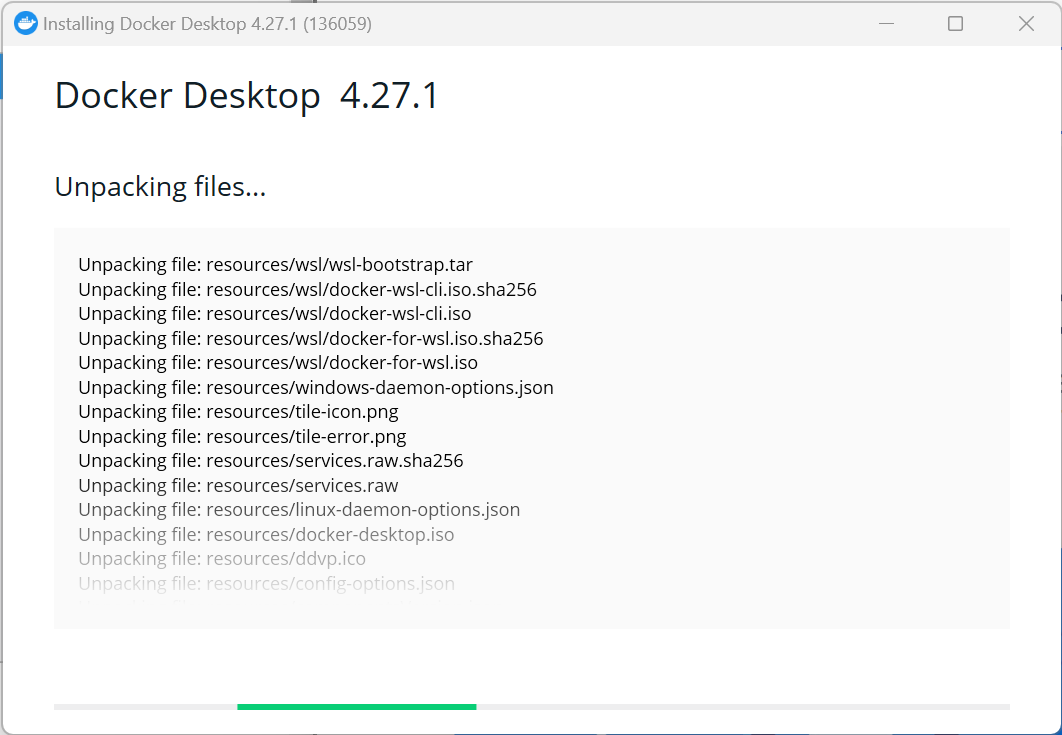
\includegraphics[width=1\linewidth]{M3_Virtualización_y_Contenedores/Tarea_3_Creación_Contenedor_Docker/reporte/figuras/2-1_Instalación_Docker.png}
    \captionof{lstlisting}{Instalación de Docker}
    \label{fig:Instalación_Docker_1}
\end{figure}

La instalación de Docker a comparación con la de Oracle VirtualBox fue mucho más sencillas, realizamos la instalación por defecto por lo que no fue requerida alguna configuración especial, como se muestra en la figura \ref{fig:Instalación_Docker_1} observamos una interfaz bastante amigable en la que por el momento no contamos ni con alguna imagen o contenedor creados.

\begin{figure}[H]
    \centering
    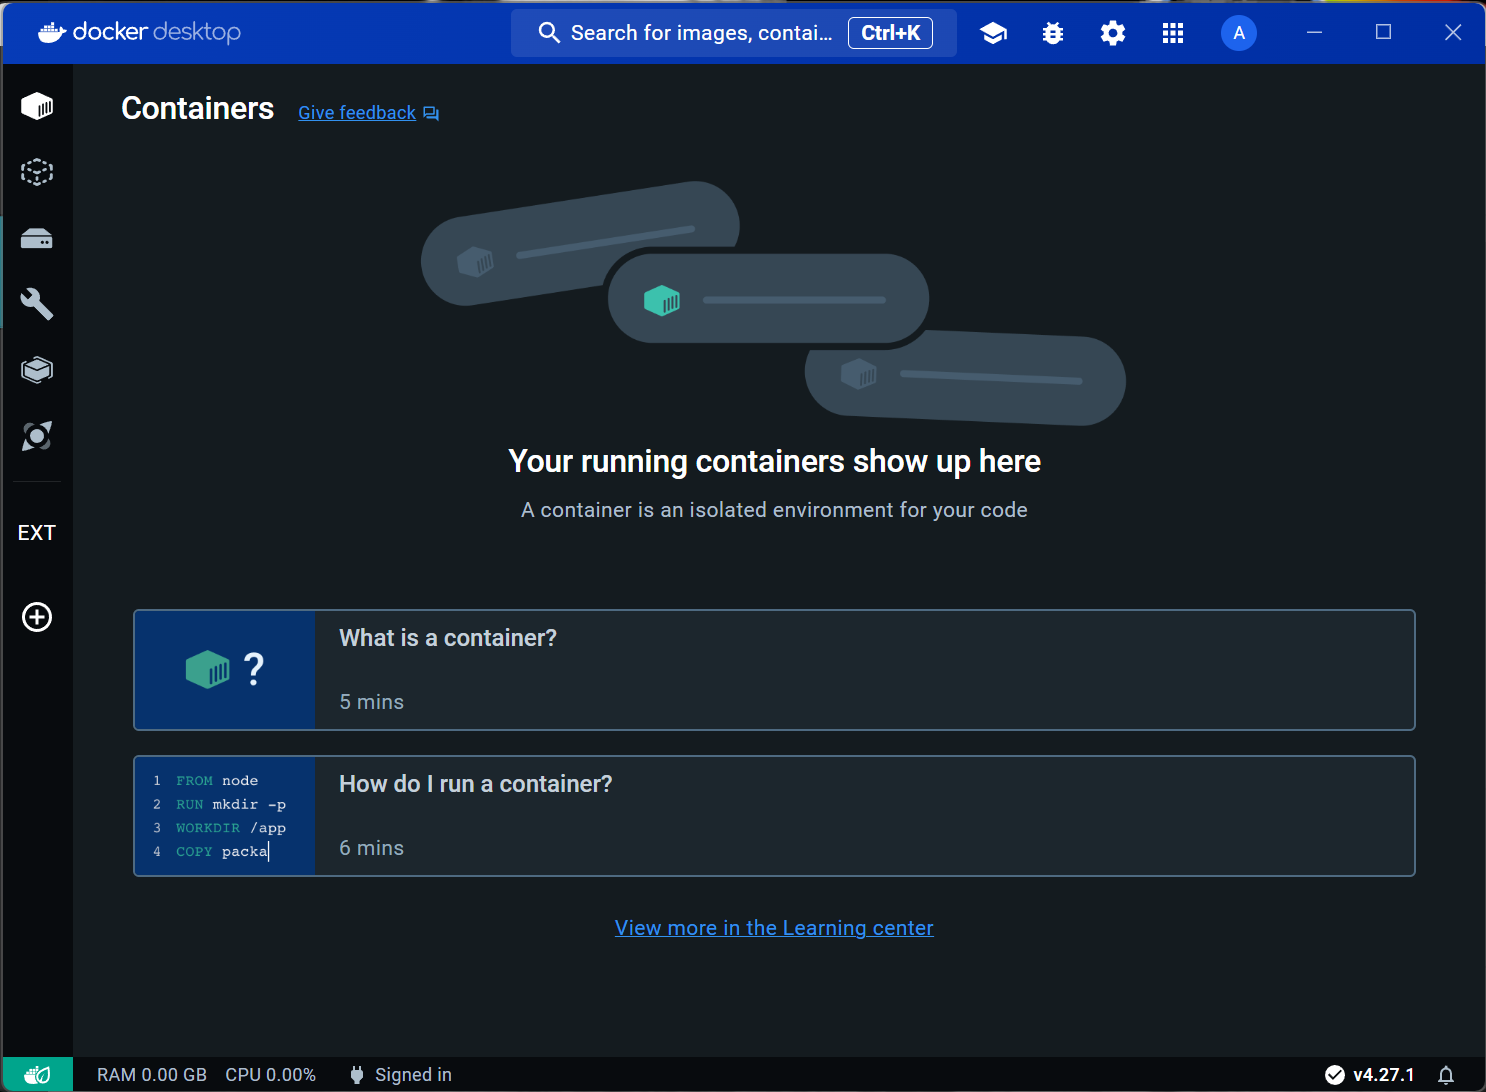
\includegraphics[width=1\linewidth]{M3_Virtualización_y_Contenedores/Tarea_3_Creación_Contenedor_Docker/reporte/figuras/2-2_Instalación_Docker.png}
    \captionof{lstlisting}{Instalación de Docker}
    \label{fig:Instalación_Docker_2}
\end{figure}


\section{Preparación del contenedor}

El siguiente paso es la preparación del contenedor donde primero creamos un archivo llamado \textbf{Dockerfile} sin extensión, este archivo lo colocamos en la carpeta donde estarán los archivos de nuestro sitio web a mostrar cuya carpeta renombramos como \textbf{public-html} y dentro del archivo colocamos el siguiente contenido:

\begin{lstlisting}[]
FROM httpd:2.4
COPY ./public-html/ /usr/local/apache2/htdocs/
\end{lstlisting}

Posteriormente procedemos a crear la imagen del servidor web a través de \textbf{Apache} utilizando el servicio \textbf{httpd} y procedes a través de la línea de comandos a ejecutar el siguiente comando:

\begin{lstlisting}[]
docker build -t apache-portafolio-web:1.0 .
\end{lstlisting}


\begin{figure}[H]
    \centering
    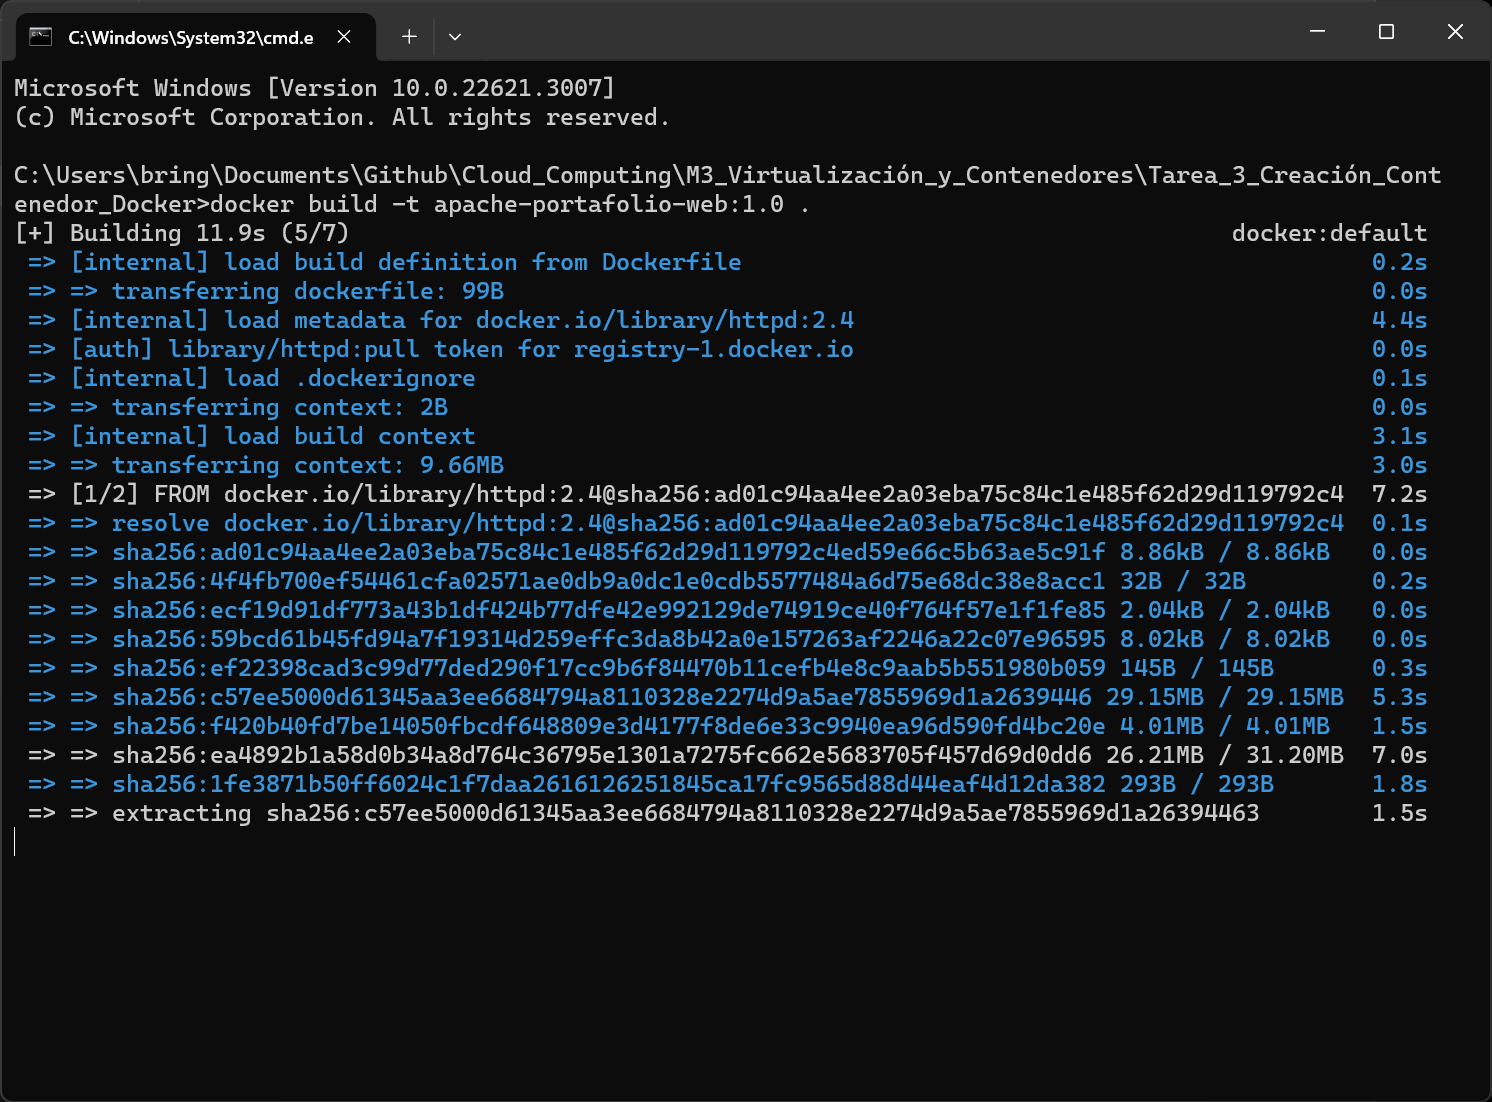
\includegraphics[width=1\linewidth]{M3_Virtualización_y_Contenedores/Tarea_3_Creación_Contenedor_Docker/reporte/figuras/3-1_Preparación_del_Contenedor.png}
    \captionof{lstlisting}{Preparación del Contenedor}
    \label{fig:Preparación_Contenedor_1}
\end{figure}

Finalmente regresamos a nuestra interfaz (GUI) de Docker desktop y observamos que la imagen creada está creada, en este caso con el nombre de \textbf{apache-portafolio-web}.

\begin{figure}[H]
    \centering
    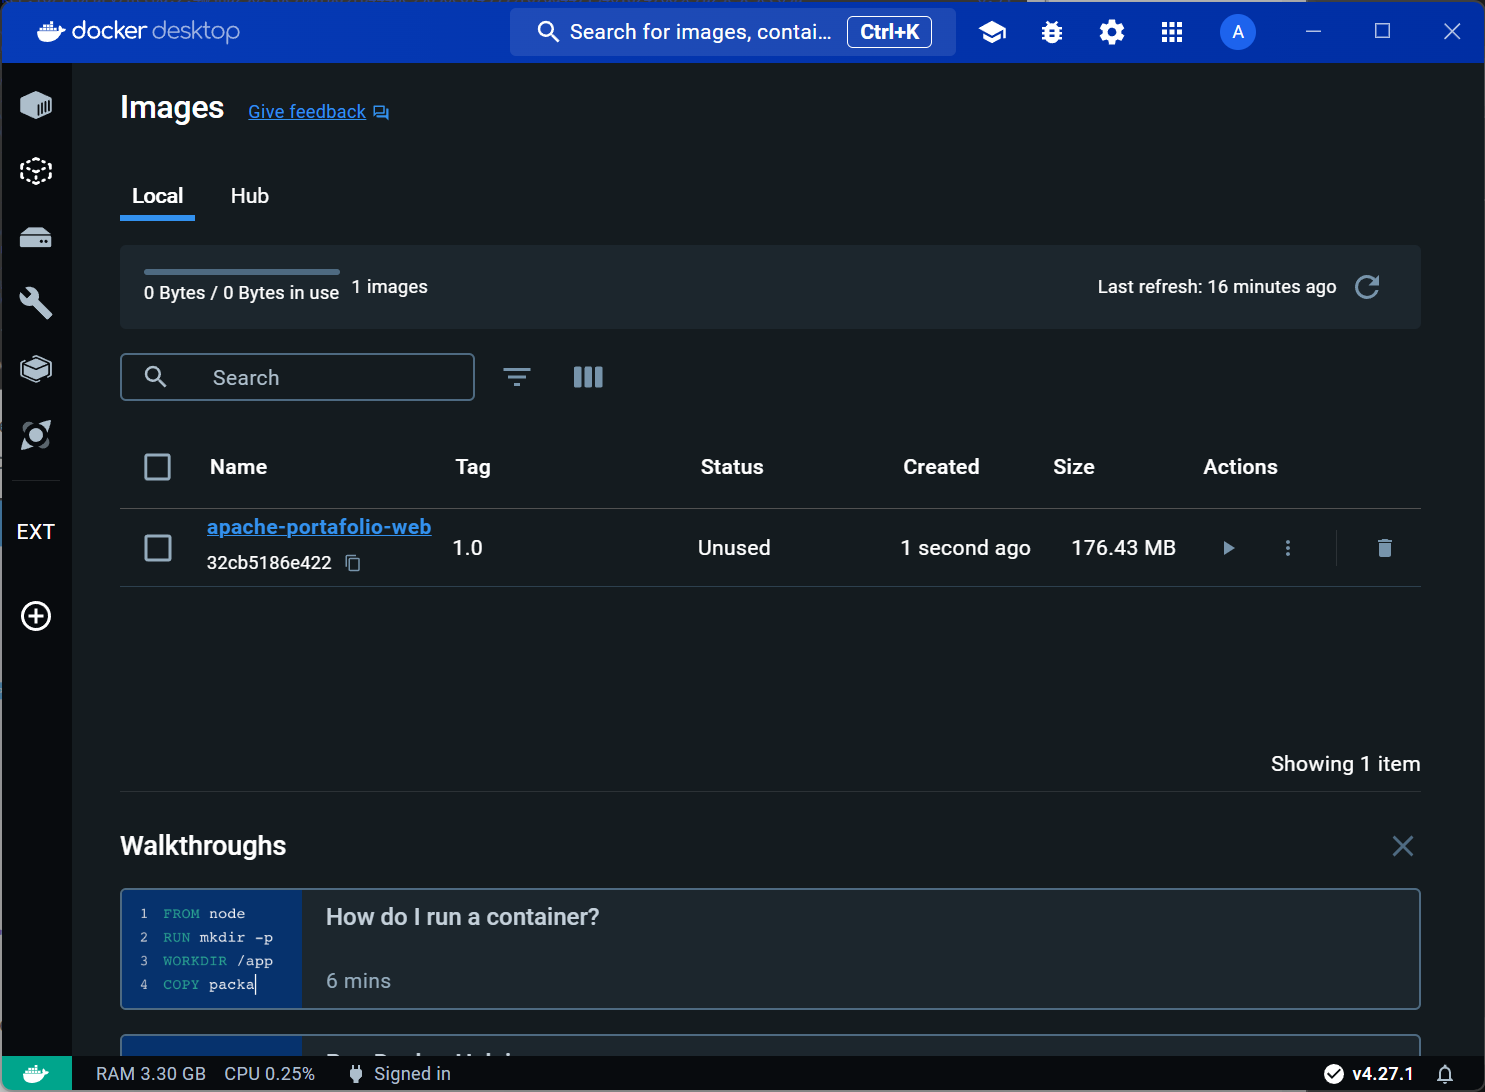
\includegraphics[width=1\linewidth]{M3_Virtualización_y_Contenedores/Tarea_3_Creación_Contenedor_Docker/reporte/figuras/3-2_Preparación_del_Contenedor.png}
    \captionof{lstlisting}{Preparación del Contenedor}
    \label{fig:Preparación_Contenedor_2}
\end{figure}


\section{Creación del contenedor}

Posteriormente procedemos a la creación del contenedor con base a la imagen que contendrá nuestro servidor web y sus archivos, esto lo hacemos ejecutando el siguiente comando en la línea de comandos:

\begin{lstlisting}[]
docker run -dit --name portafolio-web-container 
-p 8080:80 apache-portafolio-web:1.0
\end{lstlisting}


\begin{figure}[H]
    \centering
    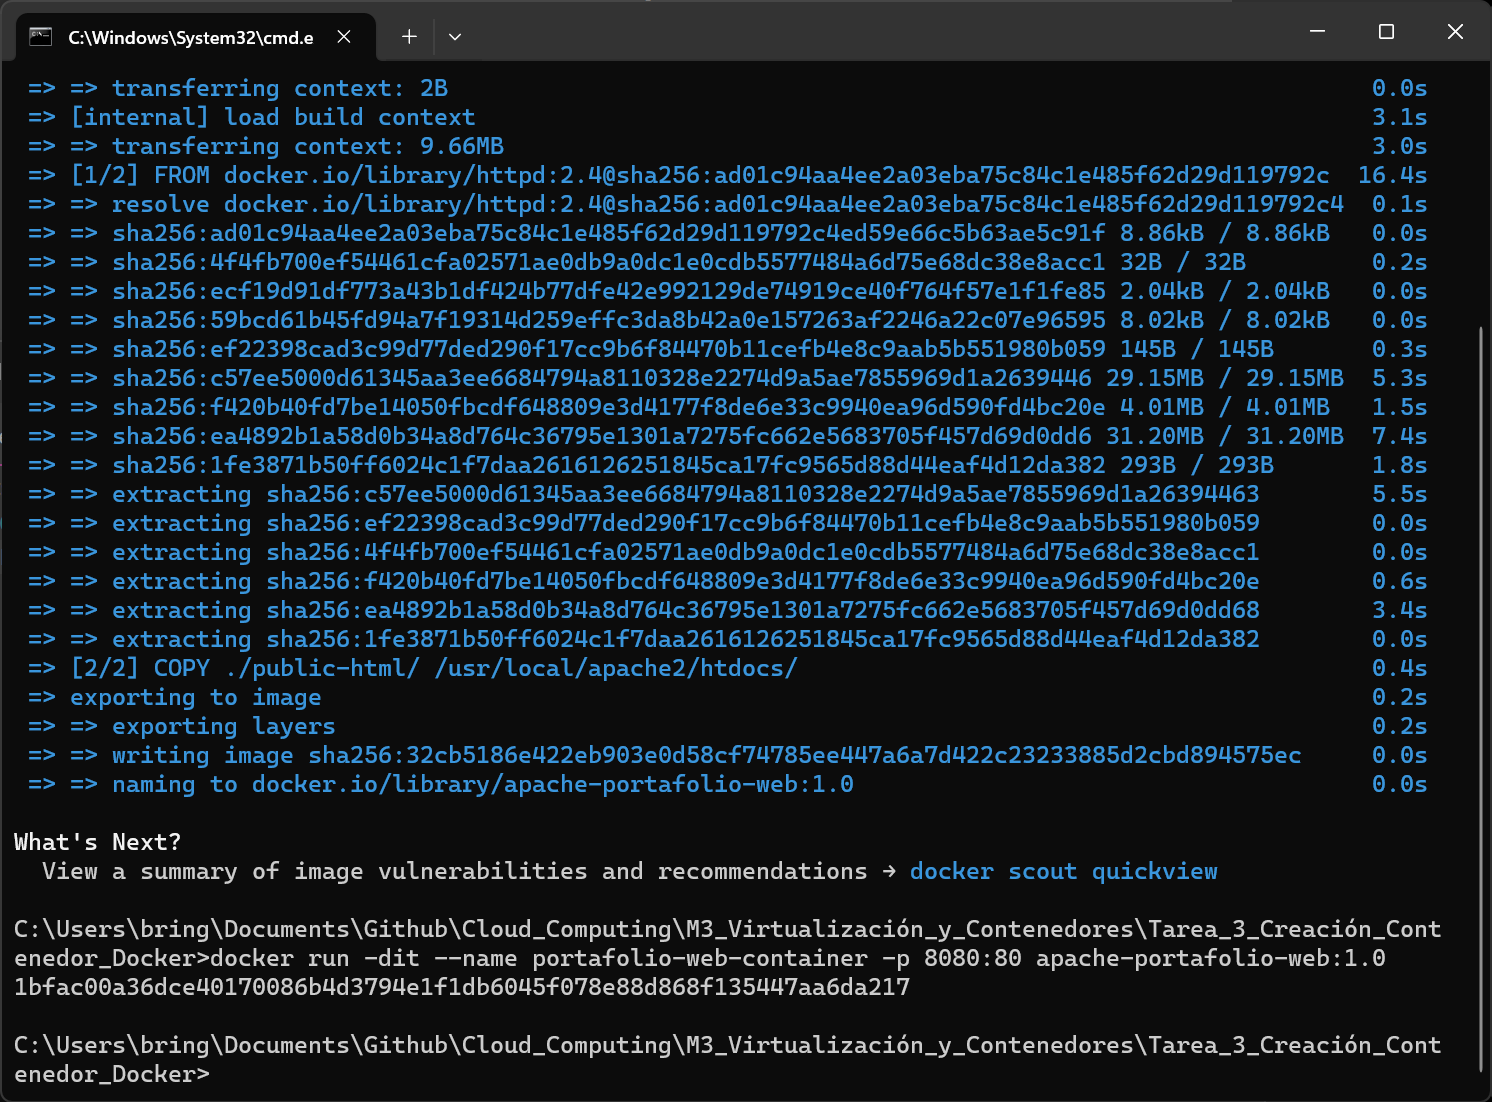
\includegraphics[width=1\linewidth]{M3_Virtualización_y_Contenedores/Tarea_3_Creación_Contenedor_Docker/reporte/figuras/4-1_Creación_del_Contenedor.png}
    \captionof{lstlisting}{Creación del Contenedor}
    \label{fig:Creación_Contenedor_1}
\end{figure}

A continuación, se da una explicación de los comandos que se utilizaron:

\begin{itemize}
    \item \textbf{docker run}: utilizado para la creación y ejecución del contenedor.
    \item \textbf{-dit}: las opciones que se utilizaron para el comando.
    \item \textbf{--name}: el nombre del contenedor, en este caso se le asigno el de \textit{portafolio-web-container}.
    \item \textbf{-p}: para redireccionar el puerto, en este caso de 8080 a 80.
    \item \textbf{apache-portafolio-web:1.0}: corresponde al nombre de la imagen que es la base para la creación que se hizo del contenedor.
\end{itemize}

En la siguiente figura \ref{fig:Creación_Contenedor_2} podemos verificar en Docker Desktop que el contenedor fue creado exitosamente.

\begin{figure}[H]
    \centering
    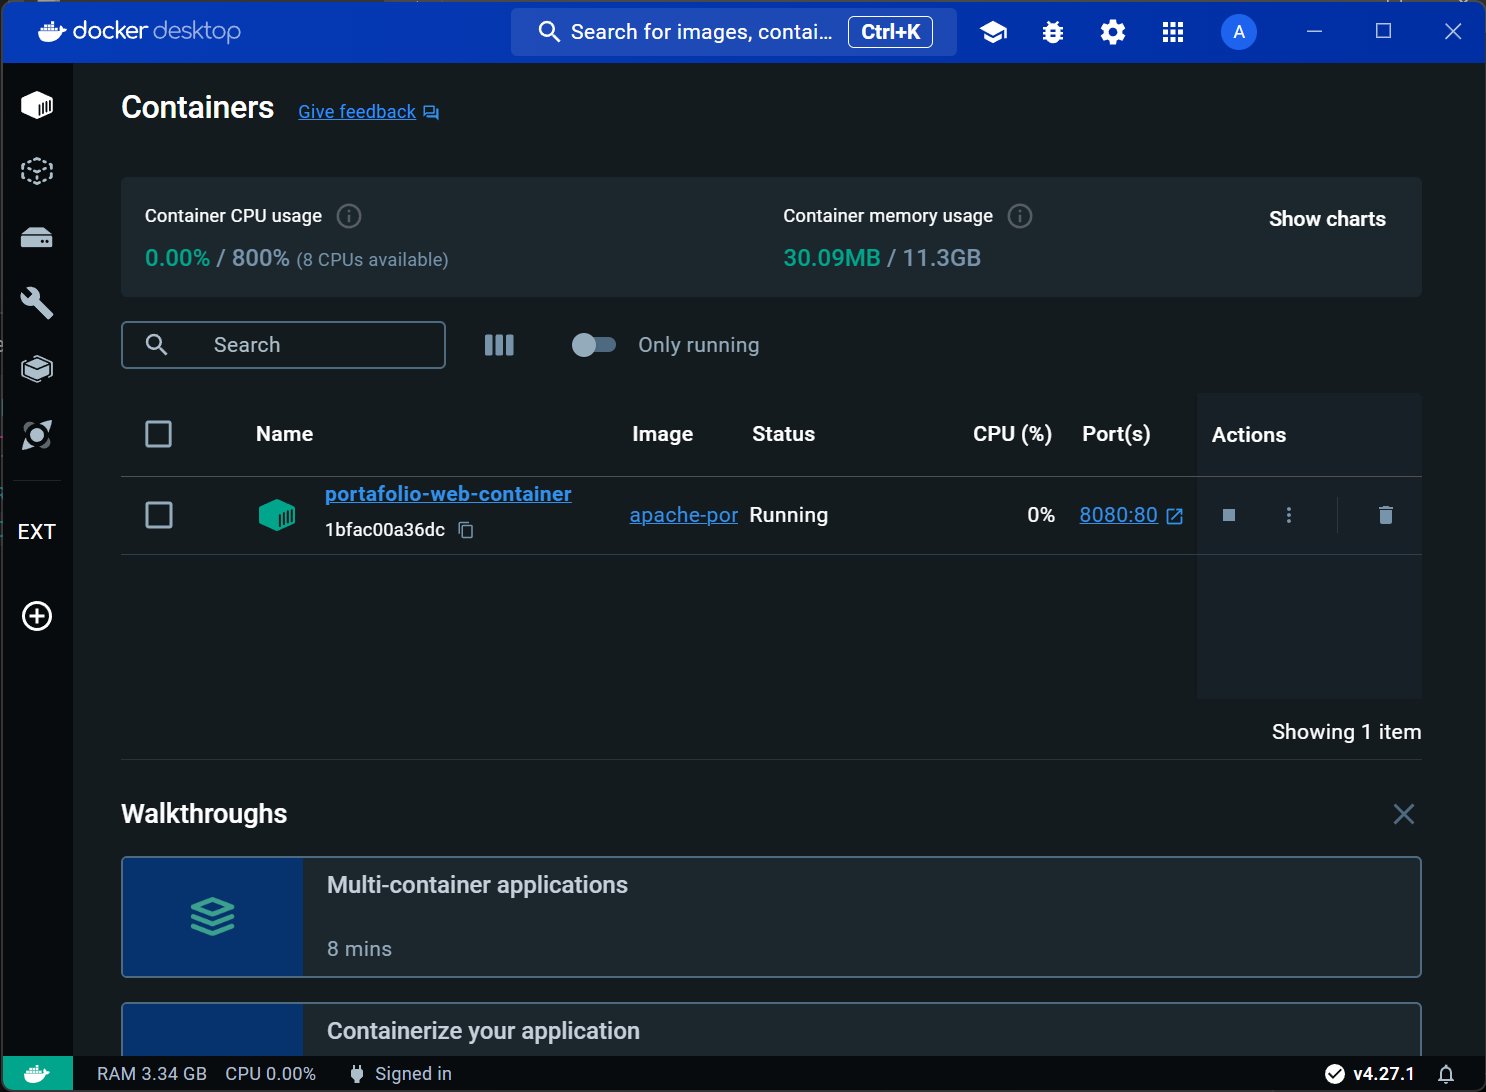
\includegraphics[width=1\linewidth]{M3_Virtualización_y_Contenedores/Tarea_3_Creación_Contenedor_Docker/reporte/figuras/4-2_Creación_del_Contenedor.png}
    \captionof{lstlisting}{Creación del Contenedor}
    \label{fig:Creación_Contenedor_2}
\end{figure}


\section{Personalización del sitio web}

Al igual que hicimos en la práctica pasada, personalizamos el sitio web como se muestra en la figura \ref{fig:Personalización_web_1} utilizando Visual Studio Code. En este caso realizamos nuevas modificaciones para que nuestro ejemplo final fuera diferente al de la práctica pasada. En la figura \ref{fig:Personalización_web_2} se pueden observar los cambios realizados en cuando a color de fondo, imagen y descripciones.

\begin{figure}[H]
    \centering
    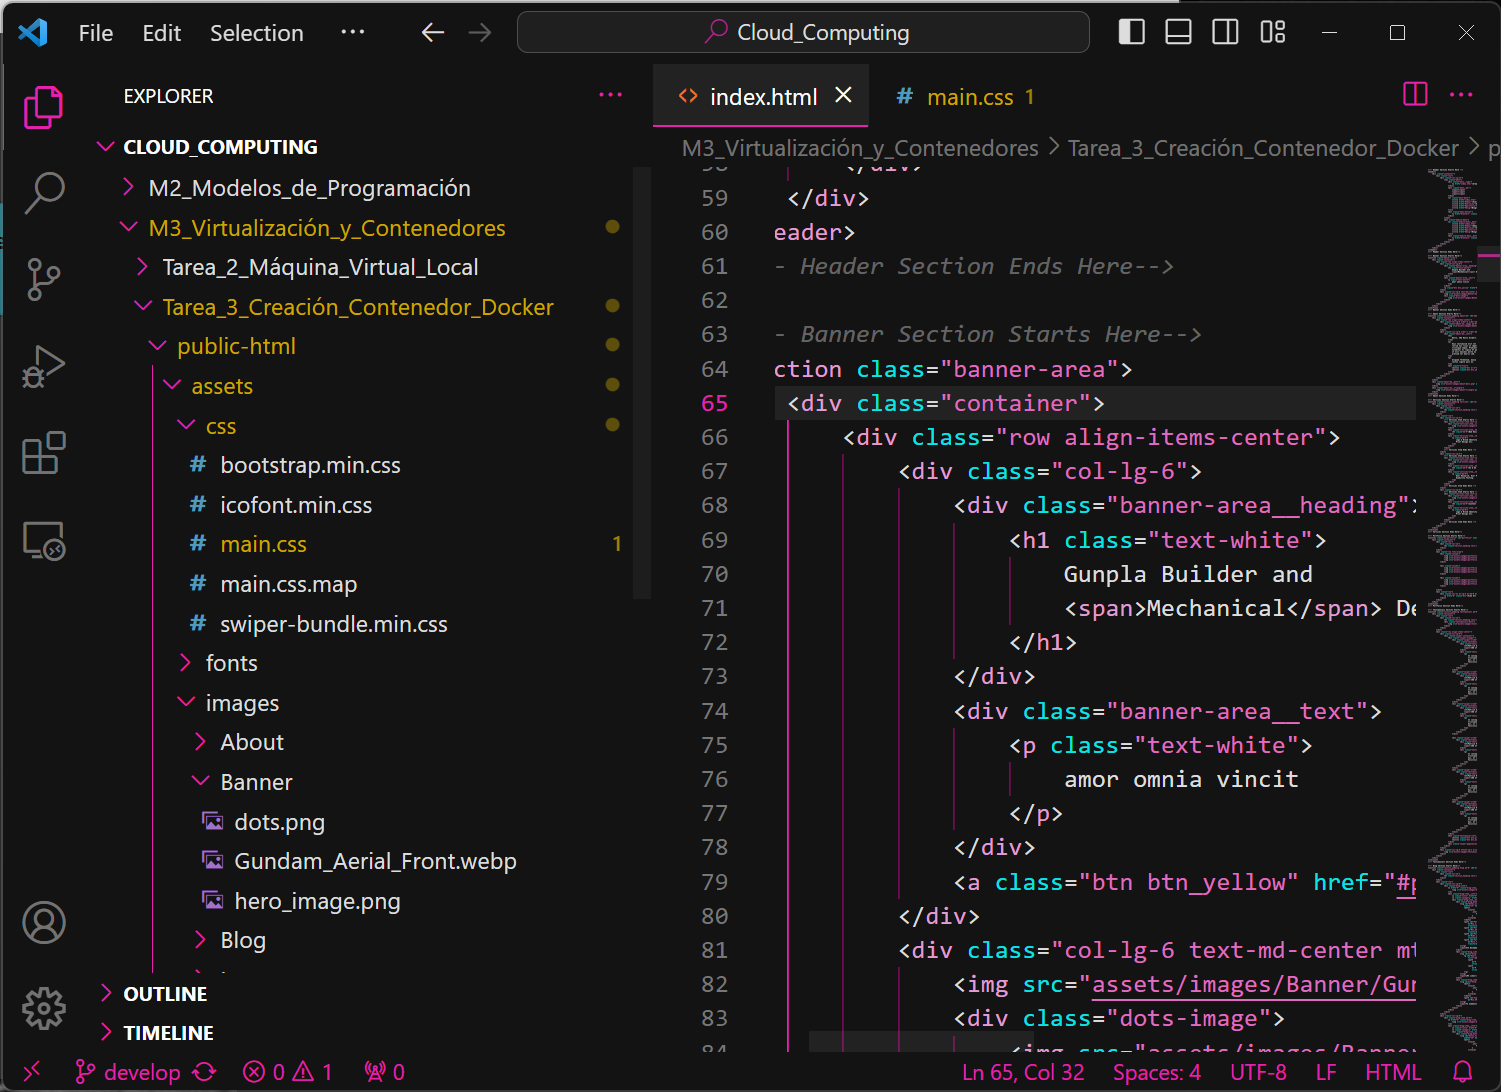
\includegraphics[width=.75\linewidth]{M3_Virtualización_y_Contenedores/Tarea_3_Creación_Contenedor_Docker/reporte/figuras/5-1_Personalización_Sitio_Web.png}
    \captionof{lstlisting}{Personalización del Sitio Web}
    \label{fig:Personalización_web_1}
\end{figure}

\begin{figure}[H]
    \centering
    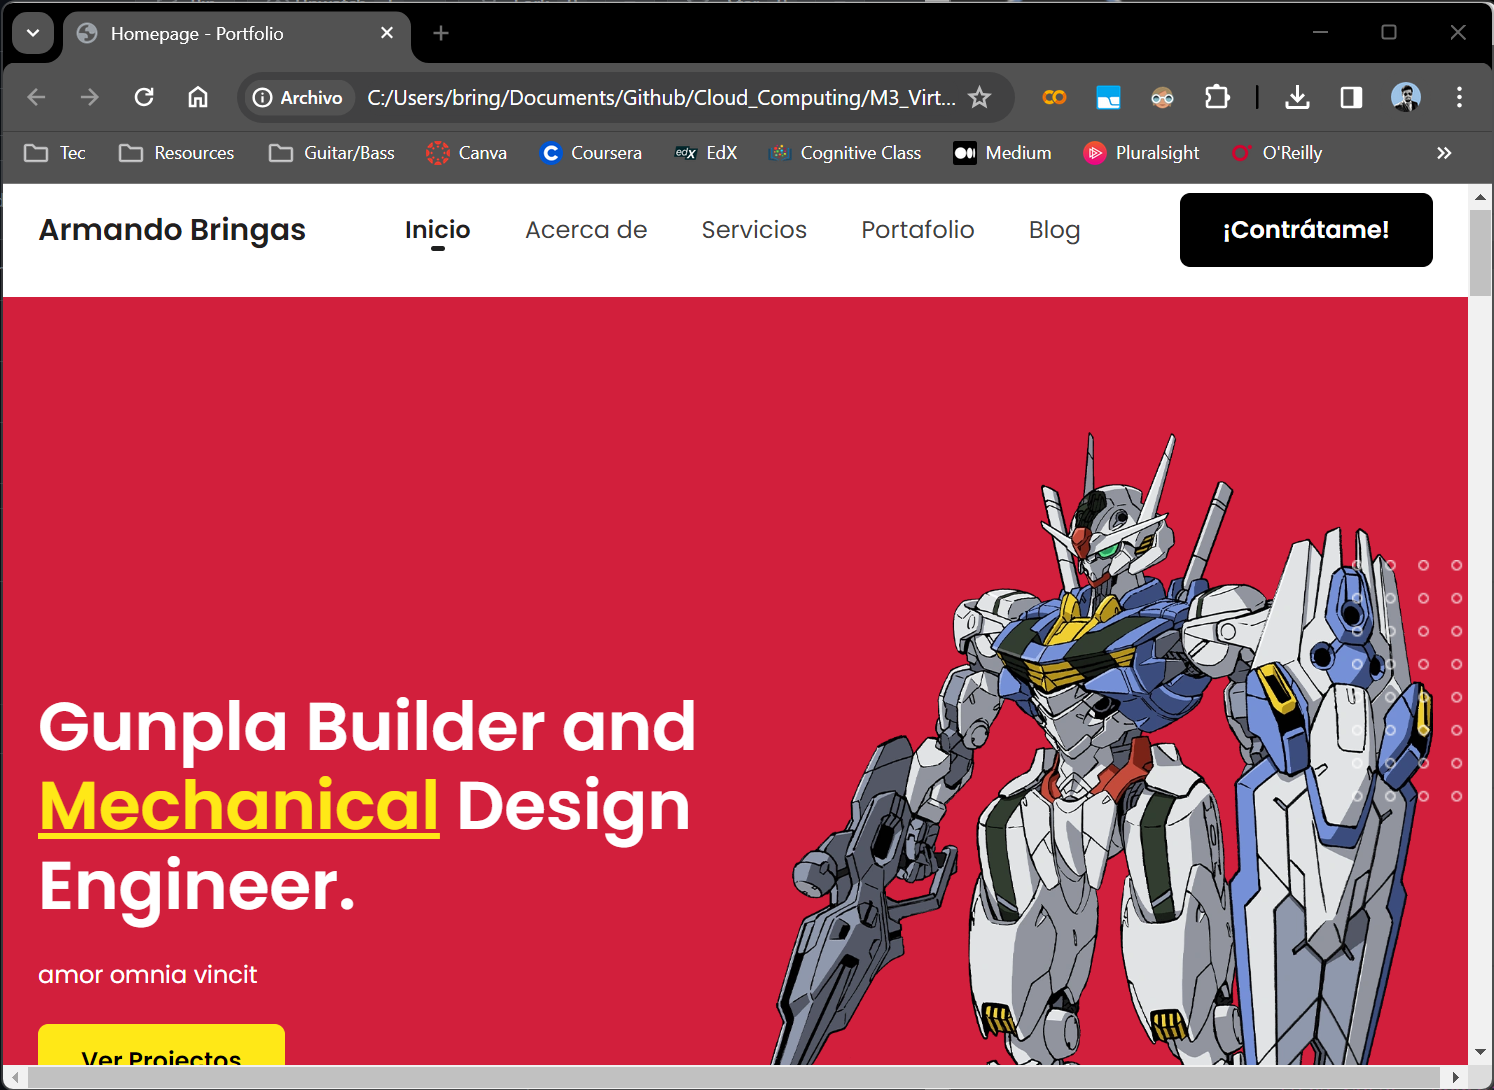
\includegraphics[width=.75\linewidth]{M3_Virtualización_y_Contenedores/Tarea_3_Creación_Contenedor_Docker/reporte/figuras/5-2_Personalización_Sitio_Web.png}
    \captionof{lstlisting}{Personalización del Sitio Web}
    \label{fig:Personalización_web_2}
\end{figure}


\section{Carga del sitio web al contenedor}

El paso final que representó el más sencillo fue desplegar el sitio web en el puerto local  que designamos cuando hicimos la creación del contenedor. En este caso no fue requerido hacer configuraciones adicionales en comparación con la práctica pasada con la Máquina Virtual en VirtualBox. En este caso lo que es importante es asegurarnos que el contenedor este activo, en caso contrario el sitio web no se desplegará.

\begin{figure}[H]
    \centering
    
\includegraphics[width=1\linewidth]{M3_Virtualización_y_Contenedores/Tarea_3_Creación_Contenedor_Docker/reporte/figuras/6-1_Carga del_Sitio_Web.png}
    \captionof{lstlisting}{Carga del Sitio Web en el Contenedor}
    \label{fig:Carga_web_1}
\end{figure}


\section{Resultados}

Finalmente, al igual que hicimos con la práctica pasada observamos que la página web se cargo de forma correcta y que funciona adecuadamente, que es responsiva y no presenta algún error al irse a alguna sección de la página web, como se puede observar en las figuras \ref{fig:Resultados_1} y \ref{fig:Resultados_2}, la renderización de la página es adecuada, por lo tanto la creación de nuestro contenedor se realizó de forma exitosa.

\begin{figure}[H]
    \centering
    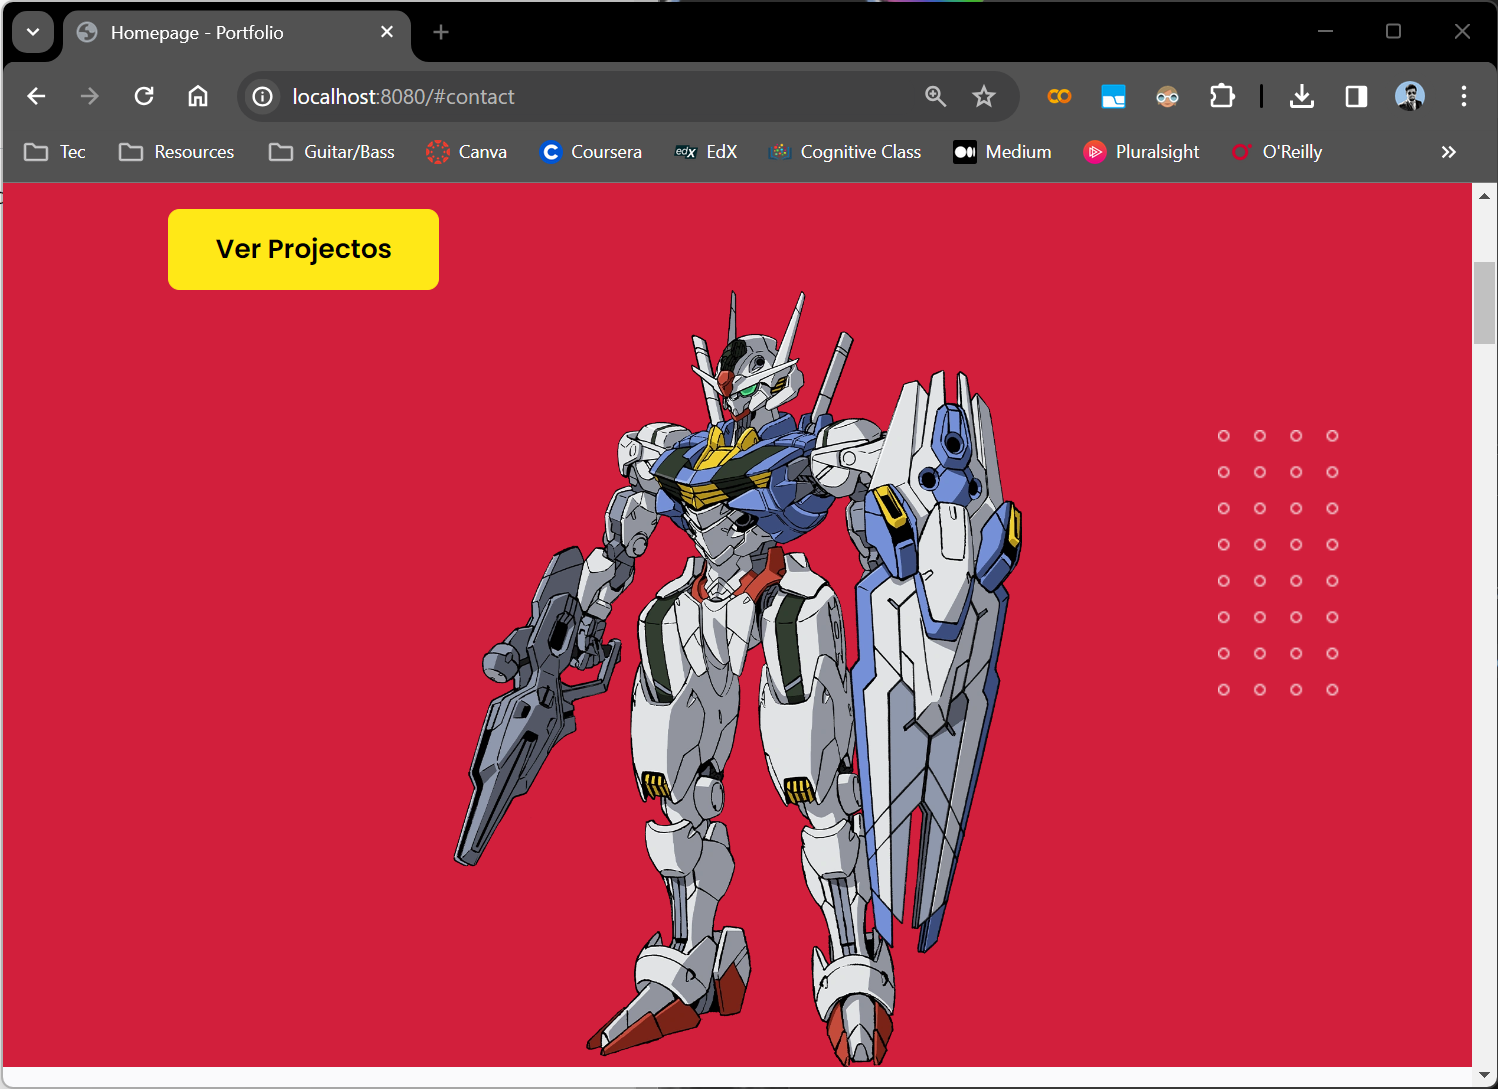
\includegraphics[width=.85\linewidth]{M3_Virtualización_y_Contenedores/Tarea_3_Creación_Contenedor_Docker/reporte/figuras/7-1_Resultados.png}
    \captionof{lstlisting}{Resultados}
    \label{fig:Resultados_1}
\end{figure}

\begin{figure}[H]
    \centering
    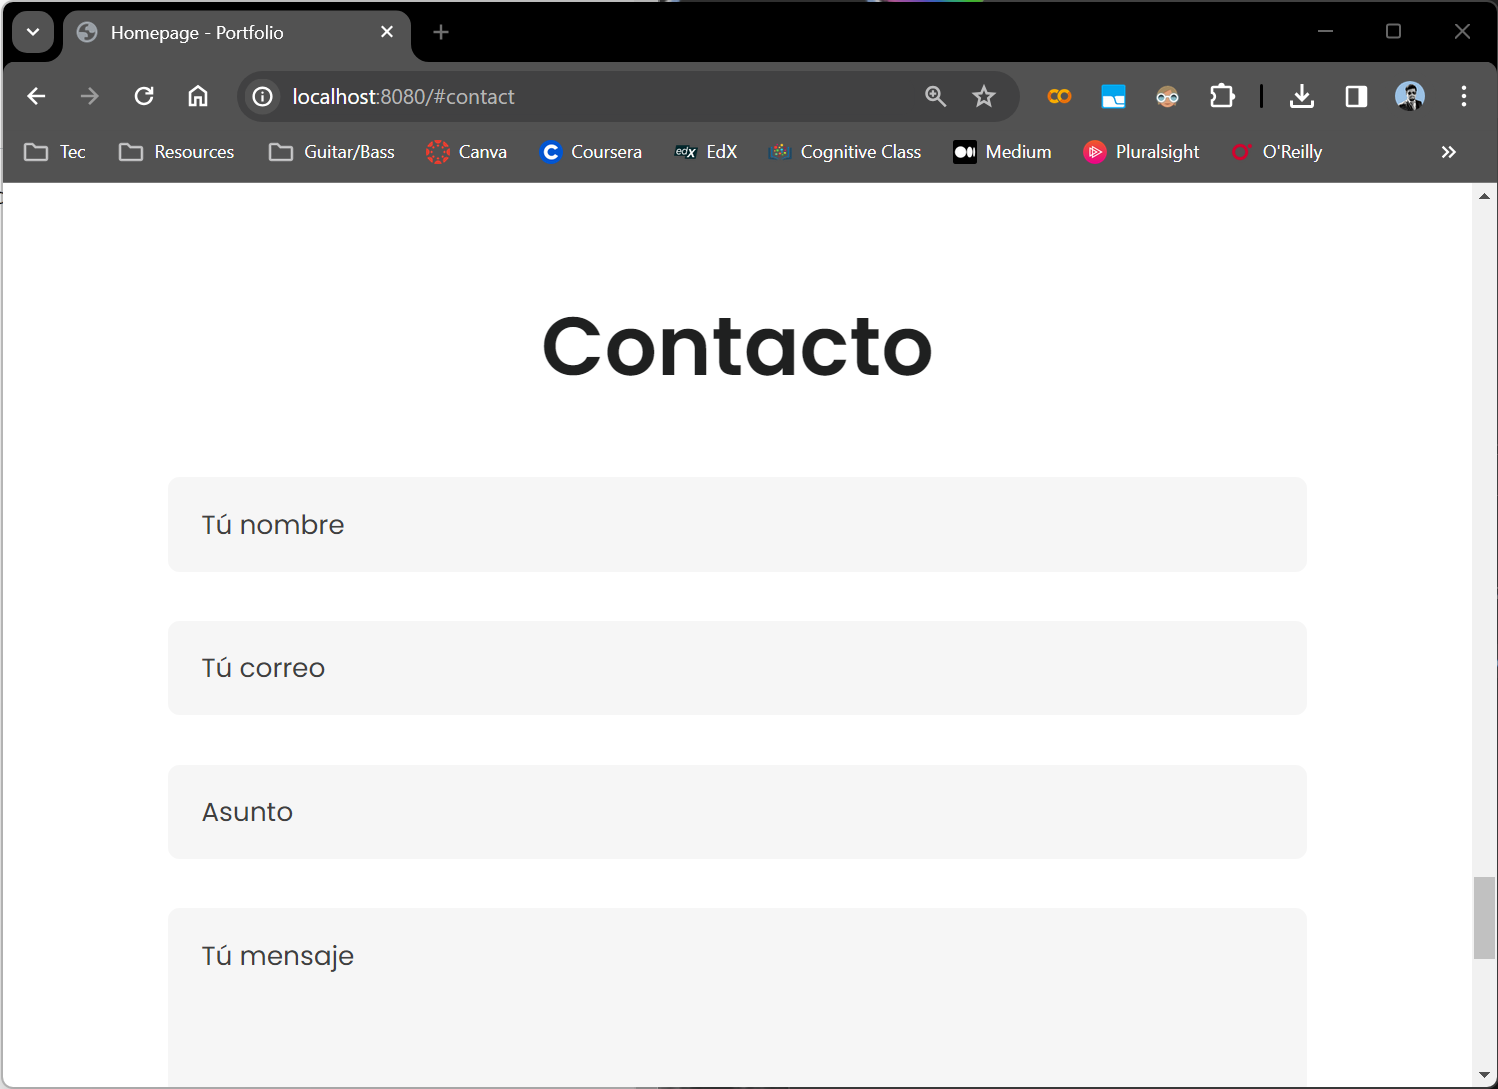
\includegraphics[width=.85\linewidth]{M3_Virtualización_y_Contenedores/Tarea_3_Creación_Contenedor_Docker/reporte/figuras/7-2_Resultados.png}
    \captionof{lstlisting}{Resultados}
    \label{fig:Resultados_2}
\end{figure}


\section{Reflexión sobre los contenedores}

En primera instancia en comparación con la práctica pasada notamos que la creación de la imagen y contenedor fue mucho más sencilla que todo el proceso de hacer una Máquina Virtual y su configuración, por otro lado vemos que los contenedores tienen como ventaja en que podemos optimizar mejor los recursos y adaptarlos a nuestras necesidades específicas.

\vspace{1em}

Otra de las ventajas que podemos observar es que podemos ejecutar varios contenedores en un solo host físico o virtual y nos necesario administrar el sistema operativo del contenedor. Quizás una desventaja es que los contenedores pueden ser menos flexibles a comparación de una Máquina Virtual cuando se busca configurar características específicas con respecto a la virtualización del hardware como memoria RAM, sistema operativo, etc. Sin embargo, los contenedores para una gran cantidad de aplicaciones son mucho más ligeros y ágiles de implementar.

\end{document}
